\pagebreak

\chapter{Memory, Buses, Priority Encoders, I/O, Floating Point, unbuffered queues}

    \section{Memory access}

        \index{memory mode}
        \index{mode!memory}
        \index{variable!memory}
        Since memory cannot be accessed in parallel it is not regarded as an
        array and is treated as a serial device which is read or written
        through one or more ports. Memory is generally available in one of
        two forms
        \blist
        \item   combinatorial output
        \item   registered output
        \blend

        Combinatorial output memory behaves when read as a combinatorial
        device - the read address is presented to the memory and the
        data at the referenced address appears at the output.

        Registered output memory only reads on the clock edge following both
        presentation of the desired address and the execution of a read
        command. Registered output memory behaves like a static variable in
        that its value (the registered output) can be used anywhere (though
        accessed by means of a function) but that value reflects the most
        recent read operation.

        Both types of memory employ clocked writes, where the address and data are
        presented to the memory and execution of a write command causes the write
        to occur.

        Memory variables are created by the inbuilt procedures -
        \begin{lstlisting}[gobble=8, language=threepl]
               cmemory(name, ports, atype, dtype, init);
               rmemory(name, ports, atype, dtype, init);
        \end{lstlisting}
        These create combinatorial output RAM and registered output RAM
        respectively. {\em name} is an identifier for the memory, {\em ports}
        (immediate) is the number of ports, {\em dtype} (immediate) is the data
        type, {\em atype} (immediate) is the address type and {\em init} is an
        optional initialisation array (immediate array variable or compound
        value). The initialisation data is a one or more dimensional
        immediate variable or structured constant whose first dimension is no
        larger than the depth of the memory. It may be smaller in which case the
        memory is zero padded. The types and structure of the initialisation
        variable or structured constant after the first dimension must match
        the memory data type. Immediate constants are padded to fit target
        elements but must not exceed the target width.

        If the initialisation argument is omitted the memory will be initialised
        to all zero. Address width is constrained by the 3PL implementation and
        by the FPGA. The implementation philosophy has been to provide an
        unrestricted data width but limit the address width since combining
        memory elements for greater depth requires more logic and introduces
        more path delays than for greater width.

        Where a memory variable is a parameter to a module, procedure or
        function only the first argument (the identifier) to {\em cmemory} or
        {\em rmemory} is needed.

        Particular FPGAs may limit the generality of some operations, e.g.
        one port may be read-only. Within this limitation multiple reads and
        writes on a port are allowed and the address and data inputs will be
        multiplexed, however there is no access arbitration and it is up to
        the application code to ensure exclusive access. Coincident accesses
        will result in data corruption.

        Each memory port may have a separate clock. The port clock is determined
        by the current clock domain when the first read or write inbuilt
        procedure/function call is executed for that port.
        
        

        \subsection{Combinatorial output memory}

            \index{memory!combinatorial output}
            A write is performed by use of the procedure {\em cmemorywrite}.
            This is called by -
            \begin{lstlisting}[gobble=12, language=threepl]
                   cmemorywrite(m, port, addr, data);
            \end{lstlisting}
            {\em m} is the memory mode variable identifier, {\em port}
            (immediate) is the memory port, {\em addr} is the address and
            {\em data} is the data to be written. {\em addr} and {\em data}
            may be immediate, value, selectvalue, static or queue modes.

            The data and address may be any type, including compound types.
            The types must match those given when the memory variable
            was created, but primitive widths may differ in which case
            padding or truncation will occur.
            
            If the address or data arguments contain queue variables the write
            will wait on queue availability.

            A read is performed by use of the function {\em cmemoryread}. This
            is called by -
            \begin{lstlisting}[gobble=12, language=threepl]
                   cmemoryread(m, port, addr)
            \end{lstlisting}
            {\em m} is the memory mode variable identifier, {\em port}
            (immediate) is the memory port and {\em addr} (immediate, value,
            selectvalue, static or queue mode) is the address.

            The address may be any type, including a compound type.
            This type must match that given when the memory variable
            was created, but primitive widths may differ in which case
            padding or truncation will occur.

            The value of the function is the data output from the read. The
            type of the function return is the data type given when the
            memory variable was created

            There may be calls to read and/or write a memory port at multiple
            points in the program, but the program logic must ensure that
            these calls are mutually exclusive (the compiler cannot determine
            that). Failure to observe this will result in data errors.
            Mutual exclusion can be enforced by the use of the {\bf waitpri}
            control structure \autorefph{sec:waitpri}.

            If both the following conditions hold -
            \blist
            \item   a port has only a single call to cmemoryread and no calls to
                    procedure cmemorywrite
            \item   the address expression contains no queues
            \blend
            then the function output will continuously (statically) reflect
            the memory contents at the requested address. This is because for
            a single read access only the address input is permanently
            connected and hence the output remains continuously valid. If the
            port has more than one access point then the address must be
            multiplexed and is only connected for the execution cycle of the
            statement in which the function call appears. For a single read
            access expressions containing a call to this function can be
            passed as arguments to modules, procedures or functions or can be
            assigned to value variables.

            If the above is not the case then the function output will only
            be valid in the execution cycle of the assignment statement in
            which the function call is part of the RHS expression, and
            expressions containing a call to this function must {\bf not} be
            passed as arguments to modules, procedures or functions or be
            assigned to value variables (the compiler will detect these and
            flag a fatal error).
            
            Note that {\bf cmemoryread()} may appear in an expression assigned
            to a value mode variable and that variable may then be used in the
            RHS of a subsequent assignment statement. There are two limitations
            to the use of {\bf cmemoryread()} in this context but -
            \blist
            \item   the value variable must be used at least once in the RHS of
                    an assignment otherwise the control logic for the memory
                    read will have no inputs
            \item   the value variable must be assigned the expression
                    containing {\bf cmemoryread()} prior to its occurrence
                    in the RHS of an assignment - post-assignment cannot
                    be used in this instance
            \blend
            These cases are recognised during immediate execution are fatal
            errors.
        
            A call to {\bf cmemorywrite()} (\autorefph{sec:ipcmemorywrite}) or {\bf cmemoryread()}
            (\autorefph{sec:ifcmemoryread}) sets the clock domain for the memory port to the
            current clock domain. All further calls to either of these inbuilt
            procedures for the same port of the same combinatorial output memory
            must be in the same clock domain (or a fatal error results).

            \subsubsection{Xilinx implementation}

                In the case of Xilinx FPGAs combinatorial output memory is
                distributed CLB RAM. This can have one or two access ports.
                One logic slice can hold 1 bit x 32 words single port or 1
                bit x 16 words dual port.

                Combinatorial output memory can be declared with an address
                width ranging from 2 (4 words) to 9 (512 words) and with any
                data width.

                Port 0 can be read or written (or both). Port 1 is read-only.


        \subsection{Registered output memory}

            \index{memory!Registered output}
            A write is performed by use of the procedure {\em rmemorywrite}.
            This is called by -
            \begin{lstlisting}[gobble=12, language=threepl]
                   rmemorywrite(m, port, addr, data);
            \end{lstlisting}
            {\em m} is the memory mode variable identifier, {\em port}
            (immediate) is the memory port, {\em addr} is the address and
            {\em data} is the data to be written. {\em addr} and {\em data}
            may be immediate, value, selectvalue, static or queue modes.

            The data and address may be any type, including compound types.
            The types must match those given when the memory variable
            was created, but primitive widths may differ in which case
            padding or truncation will occur.
            
            If the address or data arguments contain queue variables the write
            will wait on queue availability.
            
            By default a write to a registered output memory port also
            writes the value into the output register, overwriting the
            previous value. \footnote{Some FPGAs support different behaviour
            in this regard which will be incorporated into 3PL at a later date.}

            A read is performed by use of the procedure {\em rmemoryread}. This
            is called by -
            \begin{lstlisting}[gobble=12, language=threepl]
                   rmemoryread(m, port, addr);
            \end{lstlisting}
            {\em m} is the memory mode variable identifier, {\em port}
            (immediate) is the memory port and {\em addr} (immediate, value,
            selectvalue, static or queue mode) is the address.

            The address may be any type, including a compound type.
            This type must match that given when the memory variable
            was created, but primitive widths may differ in which case
            padding or truncation will occur.
            
            If the address argument contains queue variables the read
            will wait on queue availability.

            A registered output memory port read latches the result in the
            output register of the memory port, so the result can be used
            after the read has been executed (not in the same execution
            cycle). The value of the memory variable port register can be
            accessed by the function
            \begin{lstlisting}[gobble=12, language=threepl]
                   rmemoryout(m, port)
            \end{lstlisting}
            where {\em m} is the memory mode variable identifier and {\em
            port} (immediate) is the memory port. This value is continuously
            valid.
        
            A call to {\bf rmemorywrite()} (\autorefph{sec:iprmemorywrite}) or {\bf rmemoryread()}
            (\autorefph{sec:iprmemoryread}) sets the clock domain for the memory port to the
            current clock domain. All further calls to either of these inbuilt
            procedures for the same port of the same registered output memory
            must be in the same clock domain (or a fatal error results).

            There may be calls to read and/or write a memory port at multiple
            points in the program, but the program logic must ensure that
            these calls are mutually exclusive (the compiler cannot determine
            that). Failure to observe this will result in data errors.
            Mutual exclusion can be enforced by the use of the {\bf waitpri}
            control structure \autorefph{sec:waitpri}.

            \subsubsection{Xilinx implementation}

                In the case of Xilinx FPGAs registered output memory is
                block RAM. This can have one or two access ports.

                For SPARTAN 2, VIRTEX and VIRTEX E the memory formats supported
                are -

                \begin{tabular}{| l | l | l |}
                \hline
                address & data & words\\
                width & width & \\
                \hline \hline
                8  & 16 & 256   \\ \hline
                9  & 8  & 512   \\ \hline
                10 & 4  & 1024  \\ \hline
                11 & 2  & 2048  \\ \hline
                12 & 1  & 4096  \\ \hline
                \end{tabular}

                For SPARTAN3, VIRTEX 2, VIRTEX 2 Pro or Virtex 4 the memory formats
                supported are -

                \begin{tabular}{| l | l | l |}
                \hline
                address & data & words\\
                width & width & \\
                \hline \hline
                9  & 36 & 512   \\ \hline
                10 & 18 & 1024  \\ \hline
                11 & 9  & 2048  \\ \hline
                12 & 4  & 4096  \\ \hline
                13 & 2  & 8192  \\ \hline
                14 & 1  & 16384 \\ \hline
                \end{tabular}

                For Virtex 5, Virtex 6, series 7 the memory formats supported are -

                \begin{tabular}{| l | l | l |}
                \hline
                address & data & words\\
                width & width & \\
                \hline \hline
                10 & 36 & 1024  \\ \hline
                11 & 18 & 2048  \\ \hline
                12 & 9  & 4096  \\ \hline
                13 & 4  & 8192  \\ \hline
                14 & 2  & 16384 \\ \hline
                15 & 1  & 32768 \\ \hline
                \end{tabular}

                Registered output memory will employ the smallest address width
                which will encompass the address type. The data may be any
                width, multiple blocks being used if the data width exceeds the
                block data width associated with the address width. Both ports
                have the same address and data widths (the physical devices
                allow these to differ).

                Either port can be read or written (or both).













    \section{Using selectvalue variables}

        \index{buses}
        \index{mode!selectvalue}
        {\em Selectvalue} mode variables implement what is usually called a
        bus in hardware parlance. A {\em
        selectvalue} variable is combinatorial, that is it does not store
        data. A {\em selectvalue} variable can be assigned values in a number
        of places in the source code but each assignment is only valid for
        one execution cycle. Multiple assignments must be mutually exclusive.
        
        A {\em selectvalue} variable is created using the {\em selectvalue()}
        inbuilt procedure (or the {\em var()} inbuilt procedure). The current clock
        is not relevant when the variable is created.
        
        A selectvalue variable is used where one of a number of values is to
        be selected.

        Selection among alternative values can be done by multiple mutually
        exclusive assignments to static or queue variables, but there are
        two reasons why this might not be satisfactory. Firstly assignment to
        variables of these modes involves a delay - the data does not become
        available in the current execution cycle. Secondly the assignment
        logic for these variable modes requires significant logic resources
        and introduces data propagation delays in carrying out the assignment
        which may exceed the time available in the clock period. These delays
        increase with the number of separate assignment statements to the
        same primitive component.

        Selection among alternative values can also be done by a {\em value}
        mode variable whose RHS expression carries out the selection, either
        by primitive boolean logic or by nested conditional operators (?:).
        This avoids the one or more execution cycle delay inherent with
        static or queue variables, since value variables are combinatorial,
        but the selection logic again requires significant logic
        resources and introduces data propagation delays which grow with the
        number of alternatives.
        
        A bus is one or more signal lines driven from one selected source
        (usually among others). If two such assignments occur in the same
        execution cycle then that is an execution error and the result is
        undefined. If in any particular execution cycle no assignment is made to
        the variable then its value is undefined.
        
        CLB logic is used to implement selectvalue variables, but if the device
        contains 3-state buffers then these can be used instead by setting the
        selectvalue variable attribute "threestate" true\footnote{The use of
        dedicated 3-state buffers and associated routing resources can
        improve utilisation of resources in the FPGA, but these specialised
        resources are not nearly as numerous as common logic blocks and hence
        they may be exhausted by over enthusiastic use of buses.}. Signal
        propagation delays through these buffers are not large and are
        independent of the number of parallel buffers, but in practice it has
        been found preferable to use CLB logic for minimum delay.
        
        A {\em selectvalue} assignment only has effect for one execution
        cycle, but it can be extended indefinitely by simply controlling
        it by a conditional ({\em when}) or a loop ({\em while} or {\em do
        while}). Although a {\em selectvalue} variable is not itself
        clocked it must have an associated clock domain. The variable output
        is defined when assigned a value. That assignment occurs within an
        execution thread for which there is an associated clock. Similarly
        the value of the selectvalue variable will be used in expressions
        which must be evaluated in that same clock domain. A selectvalue
        variable has a clock domain established on the first assignment or
        evaluation encountered during immediate execution. All further
        assignments or evaluations must be in the same clock domain.
        
        The following example selects from among 4 inputs which are a mixture
        of variables and constants -
        \begin{lstlisting}[gobble=8, language=threepl]
               str(dtype, "uint:8");
               var(busd, selectvalue, dtype);
               static(a, dtype);
               queue(b, dtype);
               static(count, "uint:3");
               value({l1, l2}, "log");
               
               when (l1)
                   busd |- a;
               when (l2)
                   busd |- 3;
               busd |-b;
               while (count != 0) par {
                   busd |- 0;
                   count--;
               }
        \end{lstlisting}
        For any execution cycles when value variable {\em l1} is true
        variable {\em busd} will have the value of static variable {\em a}.
        For any execution cycles when value variable {\em l2} is true
        variable {\em busd} will have the value constant 3. For any execution
        cycles when queue variable {\em p} is available variable {\em busd}
        will have the value read from that queue. For any execution cycles
        when static variable {\em count} is non-zero {\em busd} will have the
        value constant 0 and {\em count} will be decremented. Any of these
        assignments may execute for a number of consecutive execution cycles,
        though in the case of the queue each execution cycle would involve a
        different datum. We assume here that these assignments will be
        mutually exclusive.

        A bus may be used to share data of a number of different types. in
        that case the bus could be created as type {\em bits} and all
        assignments cast to that type, e.g.
        \begin{lstlisting}[gobble=8, language=threepl]
               str(btype, "bits:8");
               var(busd, selectvalue, btype);
               static(a, "int:6");
               value(b, "uint:4");
               
               when (...)
                   a |- cast(a, dtype);
               when (...)
                   a |- cast(b, dtype);
        \end{lstlisting}
        Note that since the RHS of each assignment has fewer bits than the LHS
        the values will be padded, in the signed case with the sign bit.










    \section{Using priority variables}\label{usepriorityvariables}

        \index{mode!priority}
        Priority encoders are implemented in 3PL by using variables of mode {\em
        priority}. A priority variable must be created using the {\em
        priority()} or {\em var()} inbuilt procedures. The type must be a
        one-dimensional array of type {\em log}. The array may be larger than
        required, unused array members being ignored.
        
        Priority mode variables are used by control structures {\bf waitpri} and
        {\bf waitprilock} - section \ref{sec:waitpri}. These
        control structures probably cover most applications of priority mode
        variables and are easier to use than the methods described
        below. The following explanation and examples are provided for an
        understanding of how these variables work.

        Although a {\em priority} variable is not itself clocked it must have an
        associated clock domain. Inputs assigned to the priority variable will
        have clock domains (they may have a null clock domain, but that would be
        unusual) and these must all have the same clock domain. Similarly the
        value of the priority variable will be used in expressions which must be
        evaluated in that same clock domain. A priority variable has a clock
        domain established on the first assignment or evaluation encountered
        during immediate execution. All further assignments or evaluations must
        be in the same clock domain.

        A priority variable is combinatorial in that its inputs are mapped to
        its outputs with no stored state, and the outputs are a function of the
        inputs within the current execution cycle (after a propagation delay).

        Inputs to the decoder are simply assigned in the same way as value
        variables using the {\bf :=} assignment statement. This connects the RHS
        value to the encoder input selected by the subscript. The priority
        outputs are continuously available as the priority variable values.
        Inputs may be assigned in any order. The priority encoder is created at
        the completion of 3PL program execution hence if more than one
        assignment is made to any input, by default the last one will be used.
        This can be changed by setting attribute "multiplein" to true in
        which case all assignments will be collected and ORed together on
        completion of immediate execution to form the input to that priority
        array member.
        
        Members of the priority variable array whose values are used must be
        assigned. Partial use of a priority variable array has been designed to
        cater for the case where the number of members is not known prior to
        immediate execution of the 3PL program. Priority variables are usually
        used for arbitration among multiple accesses to a resource where mutual
        exclusion is required but not observed.

        For a first example suppose we wish to take the outputs of four queues
        and write them to another queue. If more than one queue is available we
        want to take them in some priority order. We could create a module
        waiting on each source queue, each one writing to the destination queue.
        Arbitration could be carried out by a global priority variable.
        \begin{lstlisting}[gobble=8, language=threepl]
               queue({sq1, sq2, sq3, sq4}, type);
               queue(dq, type);
               priority(pri);  // default type is "[20]log"
               int(pri_index);
               .
               .
               write_queue(sq1);
               write_queue(sq2);
               write_queue(sq3);
               write_queue(sq4);
               .
               .
               module
               write_queue (queue(p)) {
                   pri[pri_index] := <p;
                   sync when (pri[pri_index]) {
                       dq <<- p;
                   }
                   pri_index++;
               }
        \end{lstlisting}
        Each immediate call to {\em write\_queue} creates a module. The first
        (immediate) statement assigns the source queue availability to the
        next array member of the priority variable. The second (target)
        statement reads the source queue when the priority variable
        array member is true. The final (immediate) statement increments the
        priority variable index ready for the next call. The source queue
        priorities will be highest for {\em sq1} to lowest for {\em sq4}. If
        we wished to specify the priority on each call we could pass it as an
        argument -
        \begin{lstlisting}[gobble=8, language=threepl]
               queue({sq1, sq2, sq3, sq4}, type);
               queue(dq, type);
               priority(pri);
               .
               .
               write_queue(sq1, 5);
               write_queue(sq2, 0);
               write_queue(sq3, 2);
               write_queue(sq4, 9);
               .
               .
               module
               write_queue (queue(p), int(priority) {
                   pri[priority] := <p;
                   sync when (pri[priority]) {
                       dq <<- p;
                   }
               }
        \end{lstlisting}










    \section{Input/output}\label{sec:input_output}

        \subsection{input and output attributes}

            Variables of mode {\bf input}, {\bf output} and {\bf clock} have
            associated attributes. The attributes are such things as package pin
            locations (loc), timing names (tnm) and output current drive
            (drive). These are set as trailing arguments to inbuilt procedures {\bf
            input()}(\autorefph{sec:ipinput}), {\bf
            output()}(\autorefph{sec:ipoutput}) or {\bf
            clock()}(\autorefph{sec:ipclock}).

            When attributes are passed to input(), output() or clock() as trailing
            arguments they may be in the form attribute=value, e.g.
            \begin{lstlisting}[gobble=12, language=threepl]
                   input(vin, type(data), loc=mezz_pins[3..7], tnm="IREG");
            \end{lstlisting}

            Alternatively the trailing arguments may be maps of attributes, e.g.
            \begin{lstlisting}[gobble=12, language=threepl]
                   var(inattr, "map", {loc=mezz_pins[3..7], tnm="IREG"});
                   input(vin, type(data), inattr);
            \end{lstlisting}

            The map variable could of course have entries assigned rather than
            initialised, or could be a combination of both, e.g.
            \begin{lstlisting}[gobble=12, language=threepl]
                   var(inattr, "map", {loc=mezz_pins[3..7]});
                   inattr["tnm"] = "IREG";
                   input(vin, type(data), inattr);
            \end{lstlisting}

            The use of a map means that common attributes may be collected in a
            map which can be used for multiple input or output mode variables but
            attributes such as {\bf loc} which are individual to particular calls
            to input() or output() can be passed separately, e.g.
            \begin{lstlisting}[gobble=12, language=threepl]
                   var(inattr, "map", {tnm="IREG", ifddelay="none"});
                   input(vin1, type(data), loc=mezza_pins[3..7], inattr);
                   input(vin2, type(data), loc=mezzb_pins[10..14], inattr);
            \end{lstlisting}
            
            Note that the inbuilt procedure {\bf attributes()} can be used to assign
            or change the attributes of a variable. With the exception of pad
            locations most attributes are only used when generating logic for input,
            output and clock mode variables at completion of immediate execution so
            they can be changed at any time during immediate execution. An exception
            is the {\bf direct} attribute for output mode variables which is used
            whenever the variable is assigned.


        \subsection{input connections}

            \index{external!input signal}
            Input connections are made by creating an input mode variable
            using inbuilt procedure {\bf input()}(\autorefph{sec:ipinput}),
            e.g. -
            \begin{lstlisting}[gobble=12, language=threepl]
                   iopins(pins, "[]str", {"A1", "B1", "B2", "B3", "C1", "C2", "D1"});
                   input(vin, "uint:4", loc=pins[2..5]);
            \end{lstlisting}
            {\bf pins} is created as a string array of pin names from which four
            are selected, matching the data width.
            
            The first argument to {\bf input()} is the identifier of the created
            input mode variable.
            
            The second argument is the type of the input mode variable.
            
            The third and following arguments are optional and are attributes to be
            set. The attributes may be passed as attribute=value pairs or within one
            or more maps. The maps have the attribute names as keys and the
            associated values are the attribute values. Attribute values may be
            integers, strings or booleans but these are all converted to upper case
            strings. If an attribute is given a single value then this attribute
            value will be applied to every pin. Alternatively the attribute value
            may be a one-dimensional array whose dimension matches the number of pins.
            The array may be within a variable or it may be a compound constant in
            braces, e.g. \\
            
            \begin{lstlisting}[gobble=12, language=threepl]
                   var(a1, "[4]str", "LVCMOS33");
                   input(vin, "uint:4", loc=pins[2..5], iostandard=a1);
            \end{lstlisting}
            
            or
            \begin{lstlisting}[gobble=12, language=threepl]
                   input(vin, "uint:2", loc=pins[2..3], iostandard={"LVCMOS33", "LVCMOS25"});
            \end{lstlisting}
                        
            The {\bf loc} attribute must be supplied and the number of pins must
            match the number of bits in the data type. The attribute can be any
            nested type as long as the primitives contained therein are only "str".
            The pins are in order LSB to MSB of the target variable. If the input
            is differential then the pins are assigned in successive pairs.

            By default all input buffers with an associated flip-flop have a small
            delay inserted to avoid a hold constraint on the clocked input data.
            This delay can be removed by setting the attribute {\bf ifddelay} to 0.
            If there is no input flip-flop extra delay can be inserted in the
            signal path by setting attribute {\bf ibufdelay}.
            
            A timing group identifier attribute {\bf tnm} can be set to a string
            value to put the input pads in a timing group. This can be used to set
            up a timing constraint between the input and some other group. For
            example to remove the input delay and set up a 10ns timing constraint
            between the input and a clock we could write -
            \begin{lstlisting}[gobble=12, language=threepl]
                   iopins(pins, "[]str", {"A1", "B1", "B2", "B3", "C1", "C2", "D1"});
                   input(vin, "uint:8", loc=pins[2..5], tnm="VPAD");
                   maxdelay("VPAD", "CLK", "10.0");
            \end{lstlisting}
            where {\bf CLK} is the timing group identifier for components driven by
            the clock in question. A timing constraint identifier will be
            generated by concatenating the two timing group names separated by an
            underscore, e.g.  {\bf TS\_VPAD\_CLK} in this case.
            \index{mode!input}

            If an input register is required the input variable can be
            assigned to a static variable on every clock cycle, e.g.
            \begin{lstlisting}[gobble=12, language=threepl]
                   iopins(pins, "[]str", {"A1", "B1", "B2", "B3", "C1", "C2", "D1"});
                   input(vin, "uint:4", loc=pins[2..5]);
                   static(v_del, "bits:4"); attributes(v_del, continuous=true, iob=true);
                   v_del <- vin;
            \end{lstlisting}
            The {\bf continuous} attribute removes the assignment from any
            execution thread and connects the static variable (register)
            clock enable to logic high. The {\bf iob} attribute tells the
            place-and-route software that the flip-flops comprising the
            static variable (register) should be placed in I/O blocks along
            with their associated pads and input buffers

            Assigning an external input variable to a static variable in this way
            is the preferred method for handling external input. The static
            variable will be clocked by a clock synchronised with the external
            data, i.e. the external clock must be the current clock when the static
            assignment is encountered during immediate execution. It is not
            necessary to place a timing constraint between the input pad and the
            static variable since the routing is the fastest available, being
            simply the direct connection inside the I/O block. A timing constraint
            could be applied just to verify that the propagation delay is
            sufficiently short to meet specifications. Note that Xilinx provide an
            optional (but default) delay in external data connections to ensure
            that there is a zero hold requirement on input flip-flops.

            \index{timing constraint}
            \index{constraint!timing}
            It is difficult to decide on a specification for an acceptable input
            timing constraint. The external data source has changed the bus data
            some time after the clock. The data and clock arrive at the FPGA with
            perhaps some skew between them (the data change would usually be
            expected to follow the clock edge after some delay). The clock arrives
            at the FPGA and, if a DLL is used, is distributed with very little
            delay within the FPGA. The clock then clocks the I/O block flip-flops.

            If external data input is to be used directly without being
            assigned to a static variable then unless the clock
            frequency is very low (say less than 5MHz) timing constraints
            should be used. The following is an example where the input data
            is passed through an adder before being assigned to a static
            variable.
            \begin{lstlisting}[gobble=12, language=threepl]
               iopins(pins, "[]str", {"A1", "B1", "B2", "C3", "C4", "D1", "D2", "E1"});
               input(data_in, "bits:8", loc=pins, tnm="DPADS");
               useclock(c);
               static(v, "bits:8"); attributes(v, continuous=true);
               v <- data_in + 3;
               maxdelay("DPADS", "C", 20.0);
            \end{lstlisting}
            Here "C" is the timing group identifier for clock {\em c}, the internal
            clock derived from the external clock to which the external data is
            synchronised. The timing group identifier can be specified by supplying a
            "tnm" attribute, otherwise it is generated automatically and is simply an
            upper case version of the clock identifier.
            
            The timing constraint says that the data paths from the input connections
            through the adder up to the static variable (actually to any logic
            clocked by clock {\em c}, which will just be the flip-flops making up the
            static variable) must be 20ns or less (including flip-flop setup time).

        \subsection{output connections}

            \index{external!output signal}
            Output connections are made by creating an output mode variable.
            As an example -
            \begin{lstlisting}[gobble=12, language=threepl]
                   iopins(pins, "[]str", {"A16", "B15", "A17", "C17"});
                   value(v, "bits:4");
                   value(enable, "log");
                   output(vout, type(v),, loc=pins);
                   when (enable)
                       vout |- v;
            \end{lstlisting}
            \index{timing constraint}
            \index{constraint!timing}
            connects the 4 bit value {\bf v} to the four pins specified.
            The logical value variable {\bf enable} drives the output
            when it is true and puts it in the high-impedance state when false.
            \footnote{In the example it would be preferable if
            variables {\bf enable} and {\bf v} were static, each with the 'iob' attribute set to
            true, and variable {\bf vout} with 'direct' attribute true. That would
            result in the static variables, or shadow versions thereof, being
            placed in IO blocks rather than in CLBs. This provides the smallest 
            clock to output delays.}
            If we do not want 3-state output we could simplify the code to -
            \begin{lstlisting}[gobble=12, language=threepl]
                   iopins(pins, "[]str", {"A16", "B15", "A17", "C17"});
                   value(v, "bits:4");
                   output(vout, type(v),, loc=pins);
                   vout := v;
            \end{lstlisting}
            or more simply
            \begin{lstlisting}[gobble=12, language=threepl]
                   iopins(pins, "[]str", {"A16", "B15", "A17", "C17"});
                   value(v, "bits:4");
                   output(,, v, loc=pins);
            \end{lstlisting}

            The inbuilt procedure {\bf output()}(\autorefph{sec:ipoutput}) has at
            least four
            arguments. The first is a variable identifier, if any, for the created
            output mode variable - it need not have an identifier if the third
            argument is provided.
            
            The second argument is the type, which also can be omitted if the third
            argument is provided.

            The third argument is an optional unconditional source for the output.
            This can be used to avoid an explicit assignment to the output mode
            variable.

            The fourth and following arguments are optional and are attributes to be
            set and are passed in asimilar way to those described above for input
            mode variables.

            Note that if the source variable to output() is static its value should
            preferably not be referenced elsewhere as that will preclude its
            implementation as pad flip-flops, internal flip-flops being used
            instead. This will adversely affect the delay between clock edge and
            external data output and will probably also lead to some data skew. To
            avoid this 3PL will automatically duplicate any flip-flops whose output
            are connected to output buffers and also to other logic. One of the
            duplicates drives the output buffer and the other the internal logic.
            Clocks, clock enables and sets/resets are connected in parallel. This
            duplication can be supressed by adding a {\bf noshadow} attribute
            with a true value.

            The preferred scenario is to drive outputs from a static variable.
            The flip-flops implementing the static variable will be located in
            the I/O blocks as long as those flip-flops are not referenced
            anywhere else in the program. This arrangement means that the
            static variable is changed on the clock edge and the data
            propagation time to the output pads via output buffers is minimal.
            It is not necessary to impose timing constraints from the clock to
            the output PADS since the propagation time cannot be changed,
            but timing constraints could be used to simply verify that the
            data propagation time is low enough.
            
            An example is-
            \begin{lstlisting}[gobble=12, language=threepl]
               iopins(pins, "[]str", {"A1", "B1", "B2", "C3", "C4", "D1", "D2", "E1"});
               static(data_out, "bits:8"); attributes(data_out, iob=true);
               output(,, data_out, loc=pins, tnm="PADS");
            \end{lstlisting}
            which creates a static variable {\em data\_out}
            and connects its output to the 8 FPGA package pins specified. The
            output source is supplied via the third argument so the output will be
            directly driven i.e. 2-state not 3-state. The drive current and slew
            rate will be the default values and the output pads will be added to a
            timing group called "PADS". The {\bf iob} attribute tells the
            place-and-route software that the flip-flops comprising the static
            variable (register) should be placed in I/O blocks along with their
            associated output buffers and pads.
            
            The following example illustrates a 3-state output -
            \begin{lstlisting}[gobble=12, language=threepl]
               iopins(pins, "[]str", {"A1", "B1", "B2", "C3", "C4", "D1", "D2", "E1"});
               static(data_out, "bits:8"); attributes(data_out, iob=true);
               value({l1, l2}, "log");
               output(o, type(data_out),, loc=pins, tnm="PADS");
               when (l1 && l2)
                   o |- data_out;
            \end{lstlisting}
            Here the output drive is controlled by logical static variables
            {\em l1} and {\em l2} - if both are true the output will be
            driven, otherwise the output will be high-impedance.
            
            If the external output is a selectvalue variable or is a value
            variable at the output of combinatorial logic then the timing
            relationship between clock driven data sources and the output pads
            may need to be constrained. The following code illustrates this -
            \begin{lstlisting}[gobble=12, language=threepl]
               useclock(c);

               iopins(pins, "[]str", {"A1", "B1", "B2", "C3", "C4", "D1", "D2", "E1"});
               value(data_out, "bits:8");
               static(v, "bits:8");
               output(,, data_out, loc=pins, tnm="PADS");

               v <- .....;
               data_out := v + 3;
               maxdelay("C", "PADS", 20.0);
            \end{lstlisting}
            \index{timing constraint}
            \index{constraint!timing}
            The value variable {\em data\_out} is created and made an external
            output with pads entered into a timing group called "PADS". The
            variable is assigned a combinatorial expression whose operands are
            a static variable whose clock domain is {\em c} and an immediate
            (constant). A timing constraint is generated which limits the time
            from any logic clocked by clock {\em c} to the output pads to
            20ns. The only flip-flops (or other clocked state devices) that
            have combinatorial paths to these output pads are the ones that
            constitute the static variable {\em v}.

        \subsection{bi-directional connections}

            \index{external!bi-directional signal}
            Bi-directional I/O is simply a combination of input and output.
            The input and output variables are separate and are connected
            to the pads by separate calls -
            \begin{lstlisting}[gobble=12, language=threepl]
               iopins(pins, "[]str", {"A16", "B15", "A17", "C17"});
               type(t, "uint:4");

               input(vin, t, loc=pins);
                   .
                   .
               value(enable, "log");
               value(data, t);
               output(vout, t,, loc=pins);
               when (enable)
                   vout |- data;
            \end{lstlisting}
            assignments or initialisation for {\bf enable} and {\bf v} are not shown.
            
            Again it is preferable to use registers on input and output -
            \begin{lstlisting}[gobble=12, language=threepl]
               iopins(pins, "[]str", {"A16", "B15", "A17", "C17"});
               type(t, "uint:4");

               static({in, out}, t); attributes({in, out}, iob=true);

               input(vin, t, loc=pins);
               in <- vin;

               value(enable, "log");
               output(vout, t,, loc=pins);
               when (enable)
                   vout |- out;
            \end{lstlisting}
            If we wanted to change the above example to include timing
            constraints it might appear as follows -
            \begin{lstlisting}[gobble=12, language=threepl]
               useclock(c);

               iopins(pins, "[]str", {"A16", "B15", "A17", "C17"});
               type(t, "uint:4");

               static({in, out}, t); attributes({in, out}, iob=true);
               attributes(in, continuous=true);

               input(vin, t, loc=pins, tnm="DPADS");
               in <- vin;

               value(enable, "log");
               output(vout, type(v),, loc=pins);
               when (enable)
                   vout |- out;

               maxdelay("C", "DPADS", 10.0);
               maxdelay("DPADS", "C", 15.0);
            \end{lstlisting}
            The tnm attribute could be applied to either the input
            mode variable or the output mode variable (if both,
            only one constraint file entry will be generated).

            \index{timing constraint}
            \index{constraint!timing}
            This code applies an output constraint of 10ns and an input constraint
            of 15ns. Note that clock variables that have been used as clock domains
            have clock timing group names assigned to them automatically. These
            timing group names are derived from the clock identifier forced to
            upper case, thus a clock {\bf clk} would have a timing group identifier
            {\bf CLK} associated with it.

        \subsection{a note on timing constraints}

            \index{timing constraint}
            \index{constraint!timing}
            The examples above have applied timing constraints between I/O
            pads and state devices such as flip-flops and memories using a
            specified clock (via the clock timing group identifier).
            
            A clock period (or frequency) is specified as an attribute to the clock
            variable. A timing group identifier may also be specified for a clock
            as an attribute, otherwise a timing group identifier will be generated
            automatically using an upper case version of the clock variable
            identifier. All state devices to which this clock is connected become
            members of the associated timing group. The clock period is applied as
            a constraint for all data paths between devices in that timing group. A
            timing constraint for data paths between devices in different timing
            groups can be applied by using the library procedure {\em maxdelay}.
            This library procedure is in the header file "xilinx/common.3pl".
            It is possible to place a static variable in another timing group so
            that different timing constraints can be applied. This is done by
            setting the attribute {\em tnm}. We could change the
            bi-directional interface code above by -
            \begin{lstlisting}[gobble=12, language=threepl]
               iopins(pins, "[]str", {"A16", "B15", "A17", "C17"});
               type(t, "uint:4");

               static({in, out}, t);
               attributes(in, tnm="groupo", iob=true);
               attributes(out, tnm="groupi", iob=true);

               input(vin, t, loc=pins, tnm="DPADS");
               in <- vin;

               value(enable, "log");
               output(vout, type(v),, loc=pins);
               when (enable)
                   vout |- out;

               maxdelay("DPADS", "group0", 15.0);
               maxdelay("group1", "DPADS", 10.0);
            \end{lstlisting}
            Now the timing constraints are explicitly between the "PADS" group
            and each of the static variables.

        \subsection{the specification of I/O voltage standard}

            \index{voltage standard}
            The examples so far have not specified the I/O voltage standard.
            The place-and-route software seems to accept I/O pads and buffers
            with no voltage standard specified, but it is preferable to
            include it. The voltage standard is another attribute which can be set
            for a clock, input or output mode variable.
            
            The attribute is "iostandard" and common values are "LVCMOS33" or
            "LVCMOS25" for 3.3v and 2.5v CMOS respectively.
    
            Another attribute commonly used when setting up timing constraints
            between I/O pads and internal state devices is "tnm".

            The attributes arguments can often be rather long. For example they
            might appear as -
            \begin{lstlisting}[gobble=12, language=threepl]
               loc=mezz_pins[3..7], iostandard="LVCMOS33", tnm="OREG"
            \end{lstlisting}
            This is somewhat verbose. A more serious difficulty is that the I/O
            standard is supplied explicitly in each case where is it usually really
            a property of the associated I/O pin. To make this process more
            convenient a number of related library procedures and functions have
            been provided in library "xilinx/common.3pl".

            I/O pins are usually specified in string or string array variables, e.g.
            \begin{lstlisting}[gobble=12, language=threepl]
               iopins(bpins, "[]str", {"A1", "B1", "A2", "C1"});
            \end{lstlisting}
            but any type can be used as long as all the primitives contained
            therein are type "str".
            
            The same can now be done by calling library procedure
            {\bf iopins()} \autorefph{sec:lpiopins} with an additional argument
            supplying the I/O standard, e.g.
            \begin{lstlisting}[gobble=12, language=threepl]
               str(v33, "LVCMOS33");
               iopins(global.apins, "[]str", {"A1", "B1", "A2", "C1"}, iostandard=v33);
               iopins(bpins, "[2][2]str", {{"A3", "B4"}, {"A4", "C5"}}, iostandard=v33);
               iopins(cpin, "str", "D1", iostandard=v33);
            \end{lstlisting}
            These calls will create string or string array variables exactly as
            before but in addition a map is created in which each pin
            designation is a key whose value is the voltage standard
            string.\footnote{The use of a string variable for the voltage
            standard argument rather than a string constant not only shortens
            the line but also means that a single value is stored (pointed to)
            for each entry in the map. If the same constant is used repeatedly
            each will be a separate value which will use more memory.}

            Library procedures clock(), input() and output() call inbuilt
            procedures clock(), input() or output() respectively to create the
            variable and then take the supplied attributes, generate constraints,
            then add the attributes to the variable. Some of the attributes are
            used by 3PL in code generation and do not result in constraints being
            generated. Tnose that cause constraints to be generated usually are
            not further used by 3PL but are still stored in the variable for any
            possible later reference (they can be examined by inbuilt functions
            {\bf attributes()}(\autorefph{sec:ifattribute} and {\bf
            attribute()}(\autorefph{sec:ifattributes}).
            
            Where a pad is bi-directional and a voltage standard is specified
            for both the input and the output only one constraint for this will
            be generated.

            Note that the inference of I/O standard is done from the actual pin
            designation strings, not from the variable containing these string,
            thus copies of sub-arrays, or even string constants, can be used as
            long as the pins have been originally entered into the I/O standards
            map by using iopins().


        \subsection{differential input and output}
        
            The following code illustrates differential input for 2-bit data -
            \begin{lstlisting}[gobble=12, language=threepl]
               iopins(pins, "[]str", {"A16", "B15", "A17", "C17"});
               type(t, "uint:2");
               static(in, t);
               input(in, t, loc=pins, differential=true);
            \end{lstlisting}
            For each bit two successive pins are used from the {\bf loc} attribute.
            The first of the pair is for the +ve input and the second for the -ve
            input.

        \subsection{clock input}
        
            For a an input clock a clock mode variable is created using library
            procedure {\bf clock()} (for internal clocks the inbuilt procedure
            input() can be used instead).
            
            Clock mode variables represent all clock signals. A clock variable
            driven by a global clock buffer can be used as the clock domain for
            logic. Other clock variables represent the input clock signal from a
            pad and intermediate clock signals connecting clock managers and clock
            buffers. These are not used for clock domains since they are not
            connected to clocked devices such as flip-flops or RAMs.
            
            The following code creates a 100MHz input clock signal -
            \begin{lstlisting}[gobble=12, language=threepl]
               iopins(c100_pin, "A16");
               clock(c100_in, frequency=100.0e6, loc=c100_pin, ibufg=true);
            \end{lstlisting}
            The frequency attribute is set to 100MHz. The {\bf ibufg} selects
            whether an IBUFG input clock buffer is to be used, the alternative
            being an IBUF\footnote{It is not clear if this attribute is
            necessary as the Xilinx software may automatically use an IBUFG
            on a clock input pad.}.
            
            In an FPGA the input clock can only be used as an input to either a
            DLL/DCM or a global clock buffer. To go directly to a clock buffer (and
            hence omit any phase correction) the library procedure {\bf
            clockbufg()} is used. This library procedure is defined in one of the
            shared platform libraries, xilinx/xc2sv.3pl or xilinx/xc3s2v4v.3pl.
            \begin{lstlisting}[gobble=12, language=threepl]
               iopins(c100_pin, "A16");
               clock(c100_in, frequency=100.0e6, loc=c100_pin, ibufg=true);
               clock(global.c100, frequency=frequency(c100_in), tnm="C100");
               clockbufg(c100 <- c100_in);
            \end{lstlisting}
            The clock {\bf c100} can now be used as a clock domain. Note that it is
            made global to ensure that it can be accessed anywhere (of course clock
            domains can be in a restricted scope if desired). A timing group name
            "C100" (same as clock variable identifier but with alphabetic characters
            changed to upper case) is automatically defined in the constraints file
            and all logic clocked with this clock will be included in that timing
            group. The clock frequency attribute will be set for the timing group in
            the constraints file from which the place-and-route software will apply
            a timing constraint.
            
            In the above example it is not necessary to set the frequency
            attribute of c100 as the procedure clockbufg() will set the
            frequency attribute of its output argument to that of its input
            argument.
            
            To align the internal clock phase with the input clock a digital
            clock manager is used. The following code implements one of these.
            \begin{lstlisting}[gobble=12, language=threepl]
               iopins(c100_pin, "E17");
               float(c100_freq, 100.0e6);
               clock(c100_in, frequency=c100_freq, loc=c100_pin, ibufg=true);
               clock(global.c100, frequency=c100_freq, tnm="C100");
               clock(c100_raw, frequency=c100_freq);
               clkdcm(clk0=c100_raw <- clkin=c100_in, clkfb=c100);
               clockbufg(c100 <- c100_raw);
            \end{lstlisting}
            
            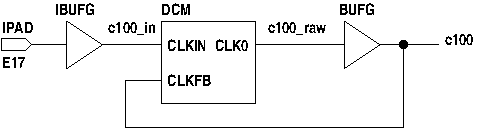
\includegraphics{dcm}
            
            To generate a divided clock as well -
            \begin{lstlisting}[gobble=12, language=threepl]
               iopins(c100_pin, "E17");
               float(c100_freq, 100.0e6);
               float(clock_ratio, 2.0);
               clock(c100_in, frequency=c100_freq, loc=c100_pin, ibufg=true);
               clock({global.c100, c100_raw}, frequency=c100_freq);
               clock({global.c50, c50_raw}, frequency=c100_freq/clock_ratio);
               attributes(c100, tnm="C100");
               attributes(c50, tnm="C50");
               clkdcm(
                   clk0=c100_raw,
                   clkdv=c50_raw
                   <-
                   clkin=c100_in,
                   clkfb=c100,
                   clkdv_divide=tostring(clock_ratio)
               );
               clockbufg(c100 <- c100_raw);
               clockbufg(c50 <- c50_raw);
            \end{lstlisting}
            
            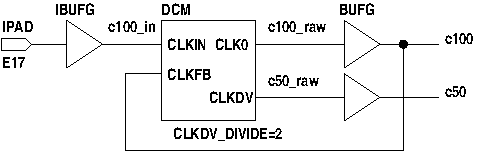
\includegraphics{dcm2}
            
            Note that in the above example the tnm attributes have been
            assigned using inbuilt procedure attributes() rather than as
            an argument to clock().

            In a CPLD the input clock can be used directly as a clock domain.

%============== THIS SECTION NEEDS TO BE CHECKED ==============================
        \subsection{DDR input}

            \index{DDR}
            For double data rate input two flip-flops are used in each IOB, one
            clocked directly and the other clocked via an inverter. The output
            of the -ve edge flip-flop must then be clocked on the next +ve edge
            into another flip-flop so that both bits are available in one clock
            domain.
            
            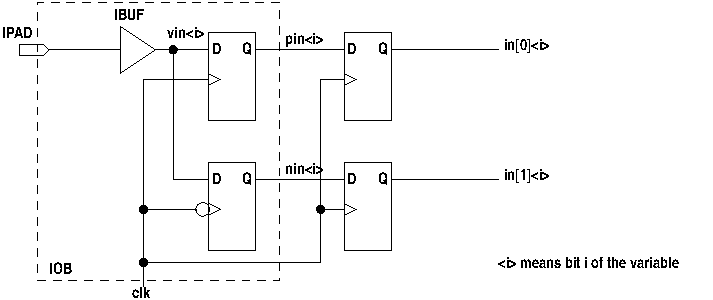
\includegraphics{ddrin}
            
            At present the Xilinx place-and-route tools accept the following
            code, but a more direct approach will be implemented shortly.

            \begin{lstlisting}[gobble=12, language=threepl]
               iopins(pins, "[]str", {"A1", "A2", "A3", "A4"});
               negclock(nclk, clk);
               input(vin, "bits:4", loc=pins);
               static(pin, "bits:4"); attributes(pin, continuous=true);
               static(nin, "bits:4"); attributes(nin, continuous=true);
               static(in, "[2]bits:4"); attributes(in, continuous=true);

               useclock(clk);
               pin <- vin;

               useclock(nclk);
               nin <- accept(vin);

               useclock(); // back to previous clock domain, clk
               in[0] <- pin;
               in[1] <- accept(nin);
            \end{lstlisting}
            When a negative clock is created using inbuilt procedure
            {\bf negclock()} the positive clock is still used but it is
            flagged such that an inverter is inserted at every logic element
            which uses it. Clock inverters are built in to all Xilinx
            clocked elements.
            
            Note the use of accept() to allow the assignment despite the different
            clock domains. It is not clear if the Xilinx place-and-route tools will
            generate and apply a half-period constraint between flip-flops clocked
            on opposite clock edges. These paths contain no logic, only routing,
            and hence tight timing constraints can be expected to be easily met.

        \subsection{DDR output}

            \index{DDR}
            For double data rate input two flip-flops are used in each IOB, one
            clocked directly and the other clocked via an inverter. The outputs
            of the two flip-flops are multiplexed to the output buffer and pad
            (using the positive clock I assume). The data must be clocked from
            two preceding flip-flops clocked with the positive clock.
            
            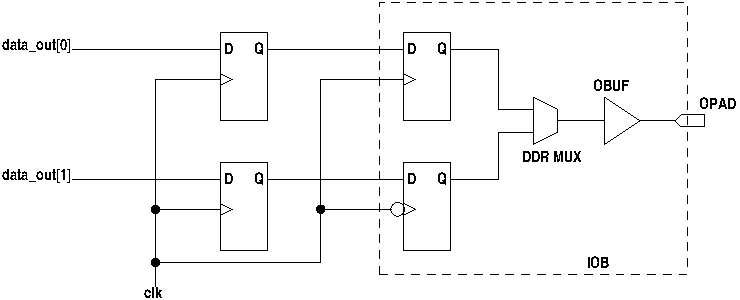
\includegraphics{ddrout}
            
            At present DDR output is not implemented, but will be shortly.


%=============================================================================



    \section{Floating point}
    
        \index{type!floating point}
        Immediate floating point values are stored in 64 bit IEEE 754 single
        precision form with a biased exponent of 8 bits and a mantissa of 23
        bits. The usual arithmetic can be used with these to form expressions.
             
        Target floating point values are stored as a struct with fields for the
        sign, biased exponent and mantissa. Thus target floating point types
        are not actually primitive.
        
        Apart from the creation of floating point variables target floating
        point is not explicitly supported by 3PL. Since target floating types
        are represented by associated structs they can be assigned to
        variables and passed as arguments to parameters. Since they are handled
        as structs the following limitations apply -
        \blist
        \item   Target floating point variables cannot be
                used in expressions. This restriction is imposed because the
                complexity of floating point operations dictates that pipelining
                should be used to achieve a reasonable throughput. Since
                operators in expressions must be capable of executing in one
                cycle if the operands are available, internal pipelining cannot
                be used by expression operators. If target floating point
                operators were implemented (which is easy enough to do) a very
                low clock frequency would have to be used to allow time for
                complete operations to be executed. The alternative adopted is
                to use library modules to carry out target floating point
                operations, these being pipelined to sustain a high throughput
                at the cost of latency.
        \item   Assignment of target floating point values cannot perform
                size adjustment and hence the left and right sides must match
                exactly in type. Where floating point sizes are to be changed
                library functions exist to do this.
        \item   Floating point parameters in modules, procedures or
                functions must either match their arguments exactly in type
                or else must have their type omitted, in which case they will
                be given the type of the argument.
        \item   Where immediate floating point arguments are passed to
                target floating point parameters the immediate values are
                converted to target floating point values with constant fields.
                These are structs of equivalent type "float:23.8". The
                parameters must either be exactly this type or else must have
                the type omitted.
        \blend
        
        For target floating point arithmetic operations there is a library,
        {\bf float.3pl} (see \autorefph{chap:fp}), which contains modules
        implementing pipelined add, subtract, multiply and divide.







    \section{Unbuffered queues}\label{sec:unbufferedqueues}
     
        \index{queue!unbuffered}
        \index{unbuffered queues}
        An unbuffered queue is one whose depth has been set to zero (by 'depth=0'
        as an attribute passed to inbuilt procedure queue() or using the {\bf
        attributes()} \autorefph{sec:ipattributes} inbuilt procedure to set it
        afterwards). For queue creation see {\bf queue()}
        \autorefph{sec:ipqueue}. These are used to synchronise two execution
        threads, optionally passing a datum in the process. A thread writing to
        an unbuffered queue will wait until a read is executed on that queue and
        vice versa. The situation is symmetrical with respect to the reader and
        writer, each waiting on the other. The read and write will execute on the
        same clock cycle.
        
        Unbuffered queues can only be synchronous, not asynchronous.
        
        Unbuffered queues cannot be initialised.
        
        An unbuffered queue may be of type "null" if no data is to be transmitted.

        An unbuffered queue cannot be read or written within -
        \blist
        \item   a {\bf waitpri} statement.
        \item   a {\bf waitprilock} statement.
        \item   a {\bf sync} statement.
        \item   a {\bf sync when} statement.
        \blend
        
        An unbuffered queue can be read or written within other control
        structures.
        
        An unbuffered queue can not be an argument to the \verb'?:' ternary
        conditional operator.
        
        A waitprilock can be used to avoid simultaneous writes to an unbuffered
        queue as long as an unbuffered queue access is not contained within
        the subject statement of the waitprilock, for example -
        
        \begin{lstlisting}[gobble=8, language=threepl]
           queue(ubq, "uint:8", depth=0);
           static(v, "uint:8");
           priority(p);

           seq {
               .
               .
               waitprilock(p, 1)
                    ;   // null subject statement
               ubq <<- 3;
               priunlock(1);
               .
           }
        \end{lstlisting}
        
        The above restrictions are required because an unbuffered queue uses
        signalling between reader and writer which is not compatible with the
        signalling used for buffered queues. When a read or write to an
        unbuffered queue is initiated that raises the available flag for the
        complementary write or read. When the complementary write or read occurs
        the opposite availability flag is briefly raised and then the read and
        write transaction is completed. If both the read and the write to an
        unbuffered queue were waiting on queue availability before proceeding then
        deadlock would occur since availability requires the initiation of the
        other side of the transaction. The second read or write operation of a
        transaction pair could employ normal synchronisation with other queues,
        but to allow this would provide too many opportunities for deadlock and
        hence the above restrictions have been imposed and enforced.
        
        An unbuffered queue can have its read or write availability tested using
        the \verb'>' or \verb'<' unary operators. Read availability will be true
        when a write is pending. In the case of a chain of assignments containing
        unbuffered queues read availability will be true when all upstream
        assignments are ready to execute and have read availability themselves.
        When an unbuffered queue has read availability its value can be examined
        using the (\verb'?' unary operator). Write availability will be true when
        a read is pending. In the case of a chain of assignments containing
        unbuffered queues write availability will be true when all downstream
        assignments are ready to execute and have write availability themselves.
        
        An assignment statement may have an unbuffered queue on the LHS and
        multiple buffered and unbuffered queues on the right hand side. The
        assignment will wait for the RHS buffered queues to be available and the
        RHS unbuffered queues to have a write pending. Reads from multiple
        unbuffered queues in an expression will wait until all unbuffered queues
        have writes able to proceed.

        An unbuffered queue may be read in more than one place and may be written
        in more than one place. In the case of multiple writers they must be
        mutually exclusive. waitprilock() statements may be used to ensure this.
        Any pending reads of an unbuffered queue will wait until a write to that
        queue after which they will continue along their execution threads.
        Unlike buffered queues the modules in which unbuffered queue reads are
        situated are not significant, i.e. unbuffered queues behave as though the
        'ignore\_modules' attribute was set (the 'ignore\_modules' attribute
        itself is ignored).

        In general unbuffered queues may be passed to modules, procedures and
        functions. Unbuffered queues cannot however be passed to inbuilt
        procedures which produce inline target code such as cmemorywrite(),
        rmemoryread() and rmemorywrite().

        Unbuffered queues are intended for synchronisation of execution threads
        usually, but not necessarily, within loops. Such loops may be implicit
        as with top level {\bf seq} or {\bf par} blocks or may be explicit
        (target {\bf while} or target {\bf do while}). The following illustrates
        a simple case -
        
        \begin{lstlisting}[gobble=8, language=threepl]
           queue(ubq, "uint:8", depth=0);
           static(v, "uint:8");

           seq {
               .
               .
               ubq <<- 3;
               .
               .
           }

           seq {
               .
               .
               v <- ubq;
               .
               .
           }
        \end{lstlisting}
        
        The first sequential thread to reach the queue access will wait for
        the other. After the write and read take place simultaneously the
        two threads will continue sequential execution and then repeat.
        
        The master-slave concept described earlier can be used to implement
        an initiation and acknowledgment scheme. A master write can be issued
        to initiate some process. The slave process waits using the read
        availablility operator. When this returns true the slave can examine
        the data using the examine operator and then execute the controlled
        operation. Meanwhile the write will hang waiting for availability.
        When the slave side has finished it can then execute a read to release
        the master write. If data is to be transfered in the other direction
        on acknowledgement then the master would be a read and the slave a
        write. An example of the former is given below -
        
        \begin{lstlisting}[gobble=8, language=threepl]
           queue(ubq, "uint:8", depth=0);

           // master thread
           static(status, type(ubq));
           seq {
               ubq <- ...;      // initiate the slave process
               .                // continue the thread
               .
               .
           }

           // slave thread
           when (<ubq) seq {
               branch (?ubq) {  // perform operations based on the examined value
               case .....
               .
               .
           }
           null <<- ubq;        // do a read to release the write in the master thread
        \end{lstlisting}
        
        By checking read availability the slave thread detects the write by the
        master thread. It then examines the written value rather than reading it,
        thus leaving the master write suspended. Finally the slave thread
        releases the master thread by doing a read. Since the data value is not
        now needed it can be dumped into null.
        
        Note that this mechanism is valid for chains of unbuffered queue
        assignments and applies to any point along that chain.
        
        Where an acknowledge status is to be returned the master reads and
        the slave writes -
        \begin{lstlisting}[gobble=8, language=threepl]
           queue(ubq, "uint:8", depth=0);

           // master thread
           static(status, type(ubq));
           seq {
               status <- ubq;   // initiate the slave process waiting for return
               .                // do something with the returned status
               .
               .
           }

           // slave thread
           when (>ubq) {
               .                // perform operations
               .
               .
               ubq <<- ...;     // return a status
           }
        \end{lstlisting}
        The master thread will initiate a read, but the queue is unavailable
        as there is no matching write from the slave. The slave however
        sees that there is write availability as a result of the master read.
        It goes ahead with thread execution and on completion writes a
        status value. The write-read transaction now completes and the master
        thread continues.

        An assigment may have multiple buffered and unbuffered queues on its
        RHS, for example -
        \begin{lstlisting}[gobble=8, language=threepl]
            type(t, "uint:8");
            queue({ubq1, ubq2}, t, depth=0);
            queue({q1, q2}, t);
            static(v, t);
           
            seq {
                .
                q1 <<- ...;
                .
            }
           
            seq {
                .
                q2 <<- ...;
                .
            }
           
            seq {
                .
                ubq1 <<- ...;
                .
            }
           
            seq {
                .
                ubq2 <<- ...;
                .
            }

            seq {
            .
                v <- q1 + ubq1 + q2 + ubq2;
                .
            }
        \end{lstlisting}
        
        The assignments to buffered queues q1 and q2 will occur when
        encountered (if these queues are not full). The assigment at the
        bottom will wait until q1 and q2 are not empty and writes are pending
        on ubq1 and ubq2. The writes to ubq1 and ubq2 will also wait until
        the last assignment statement is able to execute. When that happens
        that last seq block will move on as will the two seq blocks containing
        the writes to ubq1 and ubq2.


